%% LyX 2.3.4.2 created this file.  For more info, see http://www.lyx.org/.
%% Do not edit unless you really know what you are doing.
\documentclass[english]{article}
\usepackage[T1]{fontenc}
\usepackage[latin9]{inputenc}
\usepackage{float}
\usepackage{graphicx}

\makeatletter

%%%%%%%%%%%%%%%%%%%%%%%%%%%%%% LyX specific LaTeX commands.
%% Because html converters don't know tabularnewline
\providecommand{\tabularnewline}{\\}
\floatstyle{ruled}
\newfloat{algorithm}{tbp}{loa}
\providecommand{\algorithmname}{Algorithm}
\floatname{algorithm}{\protect\algorithmname}

%%%%%%%%%%%%%%%%%%%%%%%%%%%%%% User specified LaTeX commands.

\newcommand{\argmin}{\mathop{\mathrm{arg\,min}}}

\makeatother

\usepackage{babel}
\begin{document}
\title{An improved multistart based method for global optimization problems}
\author{Ioannis G. Tsoulos\thanks{Corresponding author. Email: itsoulos@uoi.gr}}
\date{Department of Informatics and Telecommunications, University of Ioannina,
Greece}
\maketitle
\begin{abstract}
The problem of locating the global minimum of a function finds application
in many scientific and real world problems. One of the most used and
simplest method to tackle this problem is the so called Multistart
method. This article proposes novel method based on the Multistart,
that utilizes a mechanism to prevent unnecessary local optimization
calls as well as an asymptotic stopping rule. The proposed method
is tested against Multistart on a wide set of well - known benchmark
optimization problems from the relevant literature and the results
are reported.
\end{abstract}
\textbf{Keywords}: Global optimization, stochastic methods, termination
rules.

\section{Introduction }

A new method for the task of locating the global minimum of a continuous
and differentiable function $f:S\rightarrow R,S\subset R^{n}$ is
introduced here. The task of locating the global optimum can be formulated
as, determine 
\begin{equation}
x^{*}=\mbox{arg}\min_{x\in S}f(x)\label{eq:eq1}
\end{equation}
with $S$: 
\[
S=\left[a_{1},b_{1}\right]\otimes\left[a_{2},b_{2}\right]\otimes\ldots\left[a_{n},b_{n}\right]
\]
Methods that discover the global minimum can be used in many areas
such as: economics \cite{global_econ1,global_econ2}, physics \cite{global_physics1,global_physics2},
chemistry \cite{global_chemistry1,global_chemistry2}, medicine \cite{global_med1,global_med2}
etc. Global optimization methods usually are divided into two main
categories: deterministic and stochastic methods. The most common
methods of the first category are the so called Interval methods \cite{interval1,interval2},
where the set $S$ is divided iteratively in subregions and some subregions
that not contain the global solution are discarded using some pre
defined criteria. On the other hand, in the second category there
are Controlled Random Search methods \cite{crs1,crs2,crs3}, Simulated
Annealing methods \cite{simann1,simann2}, Differential Evolution
methods \cite{diffe1,diffe2}, Particle Swarm Optimization methods
\cite{pso1,pso2}, Ant Colony Optimization \cite{aco1,aco2}, Genetic
algorithms \cite{ga1,ga2,ga3} etc. 

This article introduces a novel method which is based on the multistart
method to discover the global minimum of continuous functions. The
method incorporates an efficient stopping rule as well as an asymptotic
criterion to prevent the algorithm from unnecessary local optimization
calls. The multistart method is one of the simplest global optimization
technique which start a local search optimizer such as BFGS from different
random points and yields the lowest discovered minimum as the global
one. Due to its simplicity the method has been used in many problems
such as the TSP problem\textbf{ }\cite{multistart-tsp}, the vehicle
routing problem \cite{multistart-vehicle}, the facility location
problem \cite{multistart_fac}, the maximum clique problem \cite{multistart_clique}
etc. The method multistart has been extended in the relevant literature
with methods aim to discover all the local minima of a function \cite{tmlsl,Salhi,minfinder},
hybrid multistart techniques \cite{mshybrid1,mshybrid2}, GRASP methods\cite{grasp},
new stopping rules \cite{msstop1,msstop2,msstop3}, parallel techniques\cite{parallel-multistart,parallel-multistart2}
etc.\textbf{ }

The rest of this article is organized as follows: in section \ref{sec:Method-description}
the proposed method is described in detail, in section \ref{sec:Experiments}
the experimental results are demonstrated and finally in section \ref{sec:Conclusions}
some conclusions and guidelines for future work are provided. 

\section{Method description \label{sec:Method-description}}

The proposed method works for a predefined number of iterations. At
every iteration a number of samples is taken in the feasible region
of the objective problem. Some of them are considered as starting
points for a local search procedure and the rest are discarded. The
method continues until the maximum number of iterations is reached
or an asymptotic termination rule is satisfied. The main steps of
the proposed algorithm are outlined in Algorithm \ref{alg:The-main-steps}.
In the following subsection the main parts of the proposed algorithm
which are the discarding procedure and the proposed stopping rule
are described in detail.

\begin{algorithm}
\caption{The main steps of the proposed algorithm.\label{alg:The-main-steps}}

\begin{enumerate}
\item \textbf{Initialization Step}
\begin{enumerate}
\item \textbf{Set} $K$, the maximum number of allowed iterations.
\item \textbf{Set} $N$, the number points that will be samples at each
iteration.
\item \textbf{Set} $r_{C}=0$, the distance for the gradient check algorithm.
\item \textbf{Set} $X^{*}=\emptyset$, the set of local minima discovered
by the local search procedure.
\end{enumerate}
\item \textbf{Main Step\label{enu:Main-Step}}
\begin{enumerate}
\item \textbf{For} $i=1..N$ \textbf{do}
\begin{enumerate}
\item \textbf{Sample} randomly a point $x\in$S.
\item \textbf{Check} if $x$ is a valid starting point for the local search
procedure using the method gradientCheck(x) given in algorithm \ref{alg:The-procedure-gradientCheck(x).}.
\item \textbf{If} gradientCheck(x)=false \textbf{then}
\begin{enumerate}
\item \textbf{Start} a local search procedure $y=L(x)$
\item \textbf{Update} the distance $r_{C}$ using the equation \ref{eq:eq2}.
\item If $x\notin X^{*}$ then $X^{*}=X^{*}\cup x$
\end{enumerate}
\item \textbf{End if}
\end{enumerate}
\item \textbf{End For}
\end{enumerate}
\item \textbf{Termination Check Step. }Check the termination rule as described
in subsection \ref{subsec:Stopping-rule}.
\begin{enumerate}
\item \textbf{If }the termination rule holds \textbf{then} terminate
\item \textbf{else goto} \ref{enu:Main-Step}
\item \textbf{End if}
\end{enumerate}
\end{enumerate}
\end{algorithm}

\begin{algorithm}
\caption{The procedure gradientCheck(x).\label{alg:The-procedure-gradientCheck(x).}}

\textbf{boolean} gradientCheck(x)
\begin{enumerate}
\item \textbf{Set} $d=\min_{y\in X^{*}}\left\Vert y-x\right\Vert $
\item \textbf{Set} $z=\arg\min_{y\in X^{*}}\left\Vert y-x\right\Vert $
\item \textbf{If} $d<r_{C}$ AND $\left(x-z\right)^{T}\left(\nabla f(x)-\nabla f(z)\right)>0$
\textbf{then return} true
\item \textbf{else return} false
\end{enumerate}
\textbf{end} gradientCheck
\end{algorithm}


\subsection{Discarding procedure}

The discarding procedure has two major elements:
\begin{itemize}
\item The first is the typical distance that is calculated after every local
search and it is given by 
\begin{equation}
r_{C}=\frac{1}{M}\sum_{i=1}^{M}\left\Vert x_{i}-x_{iL}\right\Vert \label{eq:eq2}
\end{equation}
where $x_{i}$ are starting points for the local search procedure
$L(x)$ and $x_{iL}$ is the outcome of $L\left(x_{i}\right)$. If
a point $x$ is close enough to an already discovered local minima
then it is highly possible that the point belongs to the so called
region of attraction of the minima. The region of attraction of a
local minimum $z$ is defined as:
\begin{equation}
A\left(z\right)=\left\{ x:x\in S,\ L(x)=z\right\} 
\end{equation}
\item The second element is a gradient check performed between a candidate
starting point and an already discovered local minimum. The value
of the objective function $f(x)$ near to an already discovered local
minimum can be calculated using:
\begin{equation}
f(x)\simeq f(z)+\frac{1}{2}\left(x-z\right)^{T}B\left(x-z\right)\label{eq:eq4}
\end{equation}
where $B$ is the Hessian matrix at the minimum $z.$ By taking gradients
in both sides of Equation \ref{eq:eq4} we obtain:
\begin{equation}
\nabla f(x)\simeq B\left(x-z\right)\label{eq:eq5}
\end{equation}
Of course equation \ref{eq:eq5} holds for any other point $y$ near
to $z$ 
\begin{equation}
\nabla f(y)\simeq B\left(y-z\right)\label{eq:eq6}
\end{equation}
By subtracting the equation $\ref{eq:eq6}$ from \ref{eq:eq5} and
by multiplying with $\left(x-y\right)^{T}$ we have the following
equation:
\begin{equation}
\left(x-y\right)^{T}\left(\nabla f(x)-\nabla f(y)\right)\simeq\left(x-y\right)^{T}B\left(x-y\right)^{T}>0\label{eq:eq7}
\end{equation}
\end{itemize}
From the above two points a criterion to reject a point $x$ from
being a starting point for the local search procedure could be the
equation \ref{eq:eq7}. Although, the point $x$ should be close enough
to some local minimum and for this purpose the equation \ref{eq:eq2}
is used as a distance measure.

\subsection{Stopping rule\label{subsec:Stopping-rule}}

A common way to terminate a global optimization procedure is to use
the maximum number of allowed iterations, i.e. terminate when $\mbox{iter}\ge K$.
Although, this may be a simple criterion but is not an efficient one
since, small values of the parameter $K$ mean that the algorithm
probably should terminate prematurely. On the other hand higher values
for this parameter require more function calls function calls and
higher computation times. The termination rule used here is derived
from \cite{psotsoulos}: At every iteration $k$ the variance of $f\left(x^{*}\right)$
is measured, where $x^{*}$is the located global minimum so far. Denote
this variance with $\sigma^{(k)}$. If there is no any new minimum
found for a number of generations, then it is highly possible that
the algorithm has found the global minimum and hence it should terminate.
The algorithm terminates when 

\begin{equation}
k\ge k_{\mbox{min}}\ \mbox{AND\ }\sigma^{(k)}\le\frac{\sigma^{\left(k_{\mbox{last}}\right)}}{2}\label{eq:termination_mine}
\end{equation}
where $k_{\mbox{last}}$ is the last iteration where a new minimum
was found and $k_{\mbox{min}}$ is a predefined minimum number of
iterations, in order to prevent the algorithm from premature termination.
In figure the values $\sigma^{(k)}$ denoted as VARIANCE and the value
$\frac{\sigma^{\left(k_{\mbox{last}}\right)}}{2}$ denoted as STOPAT
are plotted. The objective function used is the EXP8 function given
by:
\begin{equation}
f(x)=-\exp\left(-0.5\sum_{i=1}^{8}x_{i}^{2}\right),\quad-1\le x_{i}\le1
\end{equation}
 The value of $k_{\mbox{min}}$ is set to 20 iterations and the maximum
number of iterations is 200. The algorithm terminates successfully
in 40 generation without spending unnecessary function calls for about
160 generations. 

\begin{figure}
\caption{Plot of variance along with the stopping quantity for the problem
of Potential with 20 atoms.\label{fig:Plot-of-variance}}

\centering{}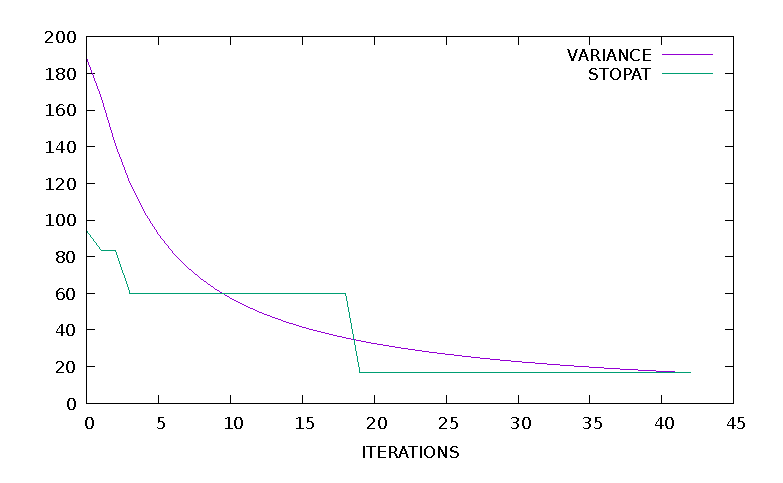
\includegraphics[scale=0.7]{termination_check}
\end{figure}


\section{Experiments\label{sec:Experiments}}

In order to measure the effectiveness of the proposed approach we
utilize several benchmark functions from the relevant literature \cite{Ali1,Floudas1}.

\subsection{Benchmark functions }

\subsubsection*{Bf1 Function }

The function Bohachevsky 1 is given by the equation

\[
f(x)=x_{1}^{2}+2x_{2}^{2}-\frac{3}{10}\cos\left(3\pi x_{1}\right)-\frac{4}{10}\cos\left(4\pi x_{2}\right)+\frac{7}{10}
\]
with $x\in[-100,100]^{2}$. The value of global minimum is 0.0.

\subsubsection*{Bf2 Function }

The function Bohachevsky 2 is given by the equation 
\[
f(x)=x_{1}^{2}+2x_{2}^{2}-\frac{3}{10}\cos\left(3\pi x_{1}\right)\cos\left(4\pi x_{2}\right)+\frac{3}{10}
\]
with $x\in[-50,50]^{2}$. The value of the global minimum is 0.0.

\subsubsection*{Branin function }

The function is defined by

$f(x)=\left(x_{2}-\frac{5.1}{4\pi^{2}}x_{1}^{2}+\frac{5}{\pi}x_{1}-6\right)^{2}+10\left(1-\frac{1}{8\pi}\right)\cos(x_{1})+10$
with $-5\le x_{1}\le10,\ 0\le x_{2}\le15$. The value of global minimum
is 0.397887.with $x\in[-10,10]^{2}$. The value of global minimum
is -0.352386.

\subsubsection*{Cosine Mixture function (CM)}

The function is given by the equation 
\[
f(x)=\sum_{i=1}^{n}x_{i}^{2}-\frac{1}{10}\sum_{i=1}^{n}\cos\left(5\pi x_{i}\right)
\]
with $x\in[-1,1]^{n}$. The value of the global minimum is -0.4 and
in our experiments we have used $n=4$.

\subsubsection*{\emph{Camel function} }

The function is given by 
\[
f(x)=4x_{1}^{2}-2.1x_{1}^{4}+\frac{1}{3}x_{1}^{6}+x_{1}x_{2}-4x_{2}^{2}+4x_{2}^{4},\quad x\in[-5,5]^{2}
\]
The global minimum has the value of $f\left(x^{*}\right)=-1.0316$

\subsubsection*{\emph{DiffPower function }}

The Sum of Different Powers function is defined 
\[
f(x)=\sum_{i=1}^{n}\left|x_{i}\right|^{i+1}
\]
and the global minimum is is $f\left(x^{*}\right)=0$. The value $n=10$
was used in the conducted experiments and the associated function
is denoted as Diffpower10.

\subsubsection*{Easom function }

The function is given by the equation 
\[
f(x)=-\cos\left(x_{1}\right)\cos\left(x_{2}\right)\exp\left(\left(x_{2}-\pi\right)^{2}-\left(x_{1}-\pi\right)^{2}\right)
\]
with $x\in[-100,100]^{2}.$ The value of the global minimum is -1.0

\subsubsection*{\emph{Exponential function}. }

The function is given by 
\[
f(x)=-\exp\left(-0.5\sum_{i=1}^{n}x_{i}^{2}\right),\quad-1\le x_{i}\le1
\]
The global minimum is located at $x^{*}=(0,0,...,0)$ with value $-1$.
In our experiments we used this function with $n=8,32$ and the corresponding
functions are denoted by the labels EXP8,EXP32.

\subsubsection*{\emph{Griewank2 function}.}

The function is given by
\[
f(x)=1+\frac{1}{200}\sum_{i=1}^{2}x_{i}^{2}-\prod_{i=1}^{2}\frac{\cos(x_{i})}{\sqrt{(i)}},\quad x\in[-100,100]^{2}
\]
The global minimum is located at the $x^{*}=(0,0,...,0)$ with value
0.

\subsubsection*{Griewank10 }

The function is given by the equation 
\[
f(x)=\sum_{i=1}^{n}\frac{x_{i}^{2}}{4000}-\prod_{i=1}^{n}\cos\left(\frac{x_{i}}{\sqrt{i}}\right)+1
\]
In our experiments we have used $n=10$ and the global minimum is
0.0 The function has several local minima in the specified range.

\subsubsection*{\emph{Gkls function}.}

$f(x)=\mbox{Gkls}(x,n,w)$, is a function with $w$ local minima,
described in \cite{gkls} with $x\in[-1,1]^{n}$ and $n$ a positive
integer between 2 and 100. The value of the global minimum is -1 and
in our experiments we have used $n=2,3$ and $w=50$. The corresponding
functions are denoted by the labels GKLS250 and GKLS350. 

\subsubsection*{Hansen function }

$f(x)=\sum_{i=1}^{5}i\cos\left[(i-1)x_{1}+i\right]\sum_{j=1}^{5}j\cos\left[(j+1)x_{2}+j\right]$,
$x\in[-10,10]^{2}$ . The global minimum of the function is -176.541793.

\subsubsection*{Hartman 3 function}

The function is given by
\[
f(x)=-\sum_{i=1}^{4}c_{i}\exp\left(-\sum_{j=1}^{3}a_{ij}\left(x_{j}-p_{ij}\right)^{2}\right)
\]
with $x\in[0,1]^{3}$ and $a=\left(\begin{array}{ccc}
3 & 10 & 30\\
0.1 & 10 & 35\\
3 & 10 & 30\\
0.1 & 10 & 35
\end{array}\right),\ c=\left(\begin{array}{c}
1\\
1.2\\
3\\
3.2
\end{array}\right)$ and
\[
p=\left(\begin{array}{ccc}
0.3689 & 0.117 & 0.2673\\
0.4699 & 0.4387 & 0.747\\
0.1091 & 0.8732 & 0.5547\\
0.03815 & 0.5743 & 0.8828
\end{array}\right)
\]
The value of global minimum is -3.862782.

\subsubsection*{Hartman6 }

$ $
\[
f(x)=-\sum_{i=1}^{4}c_{i}\exp\left(-\sum_{j=1}^{6}a_{ij}\left(x_{j}-p_{ij}\right)^{2}\right)
\]

with $x\in[0,1]^{6}$ and $a=\left(\begin{array}{cccccc}
10 & 3 & 17 & 3.5 & 1.7 & 8\\
0.05 & 10 & 17 & 0.1 & 8 & 14\\
3 & 3.5 & 1.7 & 10 & 17 & 8\\
17 & 8 & 0.05 & 10 & 0.1 & 14
\end{array}\right),\ c=\left(\begin{array}{c}
1\\
1.2\\
3\\
3.2
\end{array}\right)$ and
\[
p=\left(\begin{array}{cccccc}
0.1312 & 0.1696 & 0.5569 & 0.0124 & 0.8283 & 0.5886\\
0.2329 & 0.4135 & 0.8307 & 0.3736 & 0.1004 & 0.9991\\
0.2348 & 0.1451 & 0.3522 & 0.2883 & 0.3047 & 0.6650\\
0.4047 & 0.8828 & 0.8732 & 0.5743 & 0.1091 & 0.0381
\end{array}\right)
\]
The value of global minimum is -3.322368.

\subsubsection*{\emph{Potential function}. }

The molecular conformation corresponding to the global minimum of
the energy of N atoms interacting via the Lennard-Jones potential\cite{Jones}
is used as a test case here. The function to be minimized is given
by:
\begin{equation}
V_{LJ}(r)=4\epsilon\left[\left(\frac{\sigma}{r}\right)^{12}-\left(\frac{\sigma}{r}\right)^{6}\right]\label{eq:potential}
\end{equation}
In the current experiments three different cases were studied: $N=5,\ 10,\ 20$

\subsubsection*{\emph{Rastrigin function}. }

The function is given by 
\[
f(x)=x_{1}^{2}+x_{2}^{2}-\cos(18x_{1})-\cos(18x_{2}),\quad x\in[-1,1]^{2}
\]
The global minimum is located at $x^{*}=(0,0)$ with value -2.0.

\subsubsection*{Shekel7 }

\[
f(x)=-\sum_{i=1}^{7}\frac{1}{(x-a_{i})(x-a_{i})^{T}+c_{i}}
\]
 with $x\in[0,10]^{4}$ and $a=\left(\begin{array}{cccc}
4 & 4 & 4 & 4\\
1 & 1 & 1 & 1\\
8 & 8 & 8 & 8\\
6 & 6 & 6 & 6\\
3 & 7 & 3 & 7\\
2 & 9 & 2 & 9\\
5 & 3 & 5 & 3
\end{array}\right),\ c=\left(\begin{array}{c}
0.1\\
0.2\\
0.2\\
0.4\\
0.4\\
0.6\\
0.3
\end{array}\right)$. The value of global minimum is -10.342378.

\subsubsection*{Shekel 5 }

\[
f(x)=-\sum_{i=1}^{5}\frac{1}{(x-a_{i})(x-a_{i})^{T}+c_{i}}
\]
 with $x\in[0,10]^{4}$ and $a=\left(\begin{array}{cccc}
4 & 4 & 4 & 4\\
1 & 1 & 1 & 1\\
8 & 8 & 8 & 8\\
6 & 6 & 6 & 6\\
3 & 7 & 3 & 7
\end{array}\right),\ c=\left(\begin{array}{c}
0.1\\
0.2\\
0.2\\
0.4\\
0.4
\end{array}\right)$. The value of global minimum is -10.107749.

\subsubsection*{Shekel 7 }

\[
f(x)=-\sum_{i=1}^{7}\frac{1}{(x-a_{i})(x-a_{i})^{T}+c_{i}}
\]
 with $x\in[0,10]^{4}$ and $a=\left(\begin{array}{cccc}
4 & 4 & 4 & 4\\
1 & 1 & 1 & 1\\
8 & 8 & 8 & 8\\
6 & 6 & 6 & 6\\
3 & 7 & 3 & 7\\
2 & 9 & 2 & 9\\
5 & 3 & 5 & 3
\end{array}\right),\ c=\left(\begin{array}{c}
0.1\\
0.2\\
0.2\\
0.4\\
0.4\\
0.6\\
0.3
\end{array}\right)$. The value of global minimum is -10.342378.

\subsubsection*{Shekel 10 }

\[
f(x)=-\sum_{i=1}^{10}\frac{1}{(x-a_{i})(x-a_{i})^{T}+c_{i}}
\]
 with $x\in[0,10]^{4}$ and $a=\left(\begin{array}{cccc}
4 & 4 & 4 & 4\\
1 & 1 & 1 & 1\\
8 & 8 & 8 & 8\\
6 & 6 & 6 & 6\\
3 & 7 & 3 & 7\\
2 & 9 & 2 & 9\\
5 & 5 & 3 & 3\\
8 & 1 & 8 & 1\\
6 & 2 & 6 & 2\\
7 & 3.6 & 7 & 3.6
\end{array}\right),\ c=\left(\begin{array}{c}
0.1\\
0.2\\
0.2\\
0.4\\
0.4\\
0.6\\
0.3\\
0.7\\
0.5\\
0.6
\end{array}\right)$. The value of global minimum is -10.536410.

\subsubsection*{\emph{Sinusoidal function}.}

The function is given by 
\[
f(x)=-\left(2.5\prod_{i=1}^{n}\sin\left(x_{i}-z\right)+\prod_{i=1}^{n}\sin\left(5\left(x_{i}-z\right)\right)\right),\quad0\le x_{i}\le\pi.
\]
The global minimum is located at $x^{*}=(2.09435,2.09435,...,2.09435)$
with $f\left(x^{*}\right)=-3.5$. In our experiments we used $n=8,32$
and $z=\frac{\pi}{6}$ and the corresponding functions are denoted
by the labels SINU8 and SINU32 respectively.

\subsubsection*{\emph{Test2N function}. }

This function is given by the equation 
\[
f(x)=\frac{1}{2}\sum_{i=1}^{n}x_{i}^{4}-16x_{i}^{2}+5x_{i},\quad x_{i}\in[-5,5].
\]
The function has $2^{n}$ in the specified range and in our experiments
we used $n=4,5,6,7$. The corresponding values of global minimum is
-156.664663 for $n=4$, -195.830829 for $n=5$, -234.996994 for $n=6$
and -274.163160 for $n=7$.

\subsubsection*{\emph{Test30N function}. }

This function is given by 
\[
f(x)=\frac{1}{10}\sin^{2}\left(3\pi x_{1}\right)\sum_{i=2}^{n-1}\left(\left(x_{i}-1\right)^{2}\left(1+\sin^{2}\left(3\pi x_{i+1}\right)\right)\right)+\left(x_{n}-1\right)^{2}\left(1+\sin^{2}\left(2\pi x_{n}\right)\right)
\]
with $x\in[-10,10]$. The function has $30^{n}$ local minima in the
specified range and we used $n=3,4$ in our experiments. The value
of global minimum for this function is 0.0

\subsection{Experimental results}

The proposed method is compared against the multistart method with
the same number of samples at every generation and the same stopping
rule and the results are reported in Table \ref{tab:Average-number-of}.
The column PROBLEM denotes the objective function, the column MULTISTART
denotes the average function calls for the multistart method and the
PROPOSED column denotes the average function calls for the proposed
method. The number in the cells denotes average function calls for
30 independent runs using different seed for the random generator
each time. The numbers in parentheses denote the fraction of runs
where the global minimum was located. If this number is missing then
the global minimum was discovered in every independent run (100\%
success). The last row in all tables (denoted by TOTAL) is the total
number of function calls for listed test problems. The parameters
used in the experiments are listed in Table \ref{tab:Parameter-values-for}.
As it is evident from the conducted experiments there is a significant
improvement in terms of function evaluations at about 80\%. 

Also, in order to measure the efficiency of the proposed method for
as the dimension of the objective functions increases an additional
experiments was conducted: The function Exponential was used with
different values of the dimension $n$ from 2 to 20. The proposed
method is tested against Multistart and the results are plotted in
Figure \ref{fig:Average-number-of}. The average function calls required
by the proposed method are in the range {[}4000,6000{]} when the Multistart
requires 5 or 6 times more function calls. 

Additionally another experiment was conducted using the Exponential
function with $n=10$ with different values for the number of samples
$N$ and the results are plotted in Figure \ref{fig:Average-number-of-1}.
Again the Multistart requires much more function calls than the proposed
method and also the Multistart function calls tends to increase very
rapidly as compared to the calls of the proposed method.

\begin{table}
\caption{Average number of function calls for the proposed functions. \label{tab:Average-number-of}}

\begin{centering}
\begin{tabular}{|c|c|c|}
\hline 
PROBLEM & MULTISTART & PROPOSED\tabularnewline
\hline 
\hline 
BF1 & 22533 & 2833\tabularnewline
\hline 
BF2 & 18809 & 2629\tabularnewline
\hline 
BRANIN & 9735 & 1753\tabularnewline
\hline 
CM4 & 27037 & 2293\tabularnewline
\hline 
CAMEL & 13688 & 1732\tabularnewline
\hline 
DIFFPOWER10 & 1194776 & 19572\tabularnewline
\hline 
EASOM & 5372 & 199\tabularnewline
\hline 
EXP8 & 12022 & 2830\tabularnewline
\hline 
EXP32 & 18294 & 3265\tabularnewline
\hline 
GKLS250 & 17333(0.77) & 2415(0.93)\tabularnewline
\hline 
GKLS350 & 10104 & 243\tabularnewline
\hline 
GRIEWANK2 & 13003 & 1786\tabularnewline
\hline 
GRIEWANK10 & 53372 & 7184\tabularnewline
\hline 
HANSEN & 15294 & 1510\tabularnewline
\hline 
HARTMAN3 & 14815 & 11463\tabularnewline
\hline 
HARTMAN6 & 19459 & 3740\tabularnewline
\hline 
POTENTIAL5 & 111631 & 49601\tabularnewline
\hline 
POTENTIAL10 & 208405 & 91094\tabularnewline
\hline 
POTENTIAL20 & 280575 & 170524(0.97)\tabularnewline
\hline 
RASTRIGIN & 16968 & 675\tabularnewline
\hline 
SHEKEL5 & 19224 & 3465\tabularnewline
\hline 
SHEKEL7 & 20985 & 2976\tabularnewline
\hline 
SHEKEL10 & 20284 & 3566\tabularnewline
\hline 
SINU8 & 21860 & 549\tabularnewline
\hline 
SINU32 & 39905 & 1296\tabularnewline
\hline 
TEST2n4 & 15938 & 2890\tabularnewline
\hline 
TEST2n5 & 18085 & 3262\tabularnewline
\hline 
TEST2n6 & 19879 & 3451\tabularnewline
\hline 
TEST2n7 & 21432 & 4002\tabularnewline
\hline 
TEST30n3 & 24450 & 10818\tabularnewline
\hline 
TEST30n4 & 26514 & 13320\tabularnewline
\hline 
\textbf{TOTAL} & \textbf{2231781} & \textbf{426666}\tabularnewline
\hline 
\end{tabular}
\par\end{centering}
\end{table}
\begin{table}

\caption{Parameter values for the experiments. \label{tab:Parameter-values-for}}

\centering{}%
\begin{tabular}{|c|c|}
\hline 
PARAMETER & VALUE\tabularnewline
\hline 
\hline 
$K$ & 200\tabularnewline
\hline 
$N$ & 25\tabularnewline
\hline 
$k_{\mbox{min}}$ & 20\tabularnewline
\hline 
\end{tabular}
\end{table}
\begin{figure}
\caption{Average number of function calls for the function Exponential.\label{fig:Average-number-of}}

\centering{}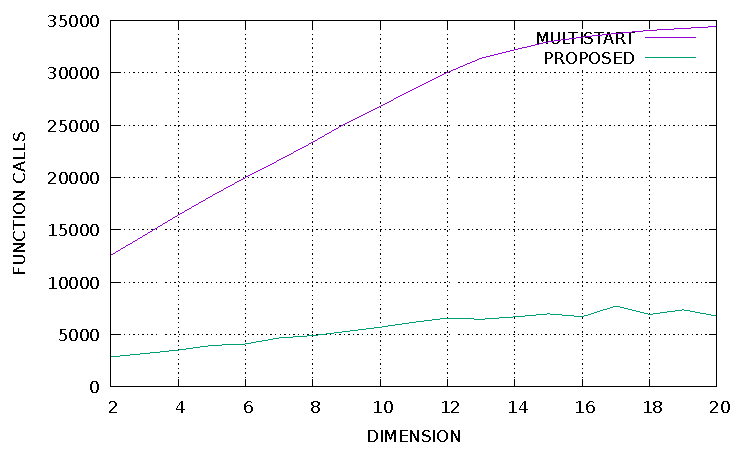
\includegraphics[scale=0.7]{expplot}
\end{figure}
\begin{figure}
\caption{Average number of function calls as the number of samples increases
for the function EXP10.\label{fig:Average-number-of-1}}

\begin{centering}
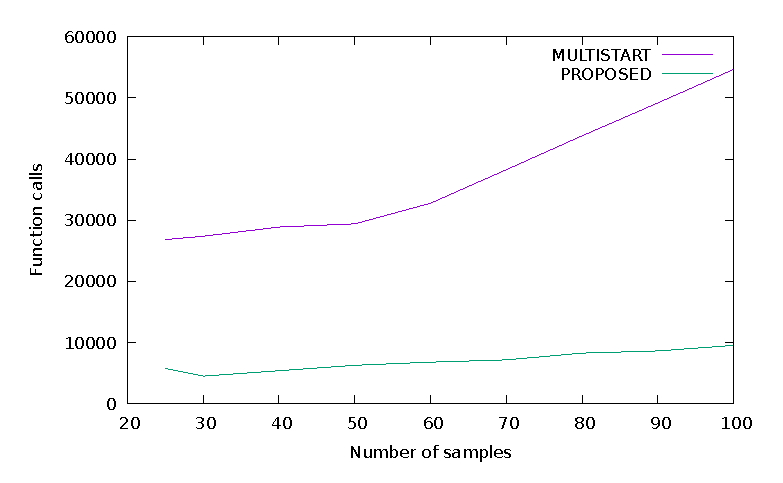
\includegraphics[scale=0.7]{plotsamples}
\par\end{centering}
\end{figure}


\section{Conclusions\label{sec:Conclusions}}

A novel multistart based method is described and tested here for global
optimization problems. The method utilizes an efficient discarding
procedure to prevent the method from unnecessary function calls and
an asymptotic stopping rule to stop the algorithm where there is a
good probability that the global optimum has been discovered. The
method was tested on a series of well known optimization problems
from the relevant literature and proved to be efficient and fast. 
\begin{thebibliography}{10}
\bibitem{global_econ1}Zwe-Lee Gaing, Particle swarm optimization
to solving the economic dispatch considering the generator constraints,
IEEE Transactions on \textbf{18} Power Systems, pp. 1187-1195, 2003.

\bibitem{global_econ2}C. D. Maranas, I. P. Androulakis, C. A. Floudas,
A. J. Berger, J. M. Mulvey, Solving long-term financial planning problems
via global optimization, Journal of Economic Dynamics and Control
\textbf{21}, pp. 1405-1425, 1997.

\bibitem{global_physics1}Q. Duan, S. Sorooshian, V. Gupta, Effective
and efficient global optimization for conceptual rainfall-runoff models,
Water Resources Research \textbf{28}, pp. 1015-1031 , 1992.

\bibitem{global_physics2}P. Charbonneau, Genetic Algorithms in Astronomy
and Astrophysics, Astrophysical Journal Supplement \textbf{101}, p.
309, 1995

\bibitem{global_chemistry1}A. Liwo, J. Lee, D.R. Ripoll, J. Pillardy,
H. A. Scheraga, Protein structure prediction by global optimization
of a potential energy function, Biophysics \textbf{96}, pp. 5482-5485,
1999.

\bibitem{global_chemistry2}P.M. Pardalos, D. Shalloway, G. Xue, Optimization
methods for computing global minima of nonconvex potential energy
functions, Journal of Global Optimization \textbf{4}, pp. 117-133,
1994.

\bibitem{global_med1}Eva K. Lee, Large-Scale Optimization-Based Classification
Models in Medicine and Biology, Annals of Biomedical Engineering \textbf{35},
pp 1095-1109, 2007.

\bibitem{global_med2}Y. Cherruault, Global optimization in biology
and medicine, Mathematical and Computer Modelling \textbf{20}, pp.
119-132, 1994.

\bibitem{interval1}M.A. Wolfe, Interval methods for global optimization,
Applied Mathematics and Computation \textbf{75}, pp. 179-206, 1996.

\bibitem{interval2}T. Csendes and D. Ratz, Subdivision Direction
Selection in Interval Methods for Global Optimization, SIAM J. Numer.
Anal. \textbf{34}, pp. 922--938, 1997. 

\bibitem{crs1}W. L. Price, Global optimization by controlled random
search, Journal of Optimization Theory and Applications \textbf{40},
pp. 333-348, 1983.

\bibitem{crs2}Ivan K\v{r}iv�, Josef Tvrd�k, The controlled random
search algorithm in optimizing regression models, Computational Statistics
\& Data Analysis \textbf{20}, pp. 229-234, 1995.

\bibitem{crs3}M.M. Ali, A. T�rn, and S. Viitanen, A Numerical Comparison
of Some Modified Controlled Random Search Algorithms, Journal of Global
Optimization \textbf{11},pp. 377--385,1997.

\bibitem{simann1}L. Ingber, Very fast simulated re-annealing, Mathematical
and Computer Modelling \textbf{12}, pp. 967-973, 1989.

\bibitem{simann2}R.W. Eglese, Simulated annealing: A tool for operational
research, Simulated annealing: A tool for operational research \textbf{46},
pp. 271-281, 1990.

\bibitem{diffe1}R. Storn, K. Price, Differential Evolution - A Simple
and Efficient Heuristic for Global Optimization over Continuous Spaces,
Journal of Global Optimization \textbf{11}, pp. 341-359, 1997.

\bibitem{diffe2}J. Liu, J. Lampinen, A Fuzzy Adaptive Differential
Evolution Algorithm. Soft Comput \textbf{9}, pp.448--462, 2005.

\bibitem{pso1}Riccardo Poli, James Kennedy kennedy, Tim Blackwell,
Particle swarm optimization An Overview, Swarm Intelligence \textbf{1},
pp 33-57, 2007. 

\bibitem{pso2}Ioan Cristian Trelea, The particle swarm optimization
algorithm: convergence analysis and parameter selection, Information
Processing Letters \textbf{85}, pp. 317-325, 2003.

\bibitem{aco1}M. Dorigo, M. Birattari and T. Stutzle, Ant colony
optimization, IEEE Computational Intelligence Magazine \textbf{1},
pp. 28-39, 2006.

\bibitem{aco2}K. Socha, M. Dorigo, Ant colony optimization for continuous
domains, European Journal of Operational Research 185, pp. 1155-1173,
2008.

\bibitem{ga1}D. Goldberg, Genetic Algorithms in Search, Optimization
and Machine Learning, Addison-Wesley Publishing Company, Reading,
Massachussets, 1989.

\bibitem{ga2}Z. Michaelewicz, Genetic Algorithms + Data Structures
= Evolution Programs. Springer - Verlag, Berlin, 1996.

\bibitem{ga3}S.A. Grady, M.Y. Hussaini, M.M. Abdullah, Placement
of wind turbines using genetic algorithms, Renewable Energy \textbf{30},
pp. 259-270, 2005.

\bibitem{multistart-tsp}Li W., A Parallel Multi-start Search Algorithm
for Dynamic Traveling Salesman Problem. In: Pardalos P.M., Rebennack
S. (eds) Experimental Algorithms. SEA 2011. Lecture Notes in Computer
Science, vol 6630. Springer, Berlin, Heidelberg, 2011.

\bibitem{multistart-vehicle}Olli Br�ysy, Geir Hasle, Wout Dullaert,
A multi-start local search algorithm for the vehicle routing problem
with time windows, European Journal of Operational Research \textbf{159},
pp. 586-605, 2004.

\bibitem{multistart_fac}Mauricio G.C. Resende, Renato F. Werneck,A
hybrid multistart heuristic for the uncapacitated facility location
problem, European Journal of Operational Research \textbf{174}, pp.
54-68, 2006.

\bibitem{multistart_clique}E. Marchiori, Genetic, Iterated and Multistart
Local Search for the Maximum Clique Problem. In: Cagnoni S., Gottlieb
J., Hart E., Middendorf M., Raidl G.R. (eds) Applications of Evolutionary
Computing. EvoWorkshops 2002. Lecture Notes in Computer Science, vol
2279. Springer, Berlin, Heidelberg. 

\bibitem{bfgs}Ya-Xiang Yuan, A Modified BFGS Algorithm for Unconstrained
Optimization, IMA Journal of Numerical Analysis \textbf{11}, pp. 325--332,
1991.

\bibitem{tmlsl}M.M. Ali, C. Storey, Topographical multilevel single
linkage, J. Global Optimization 5 (1994) 349--358

\bibitem{Salhi}S. Salhi, N.M. Queen, A hybrid algorithm for identifying
global and local minima when optimizing functions with many minima,
European J. Oper. Res. 155(2004) 51--67.

\bibitem{minfinder}I. G. Tsoulos and I. E. Lagaris, MinFinder: Locating
all the local minima of a function, Computer Physics Communications
\textbf{174}, pp. 166-179, 2006. 

\bibitem{mshybrid1}M. Perez, F. Almeida and J. M. Moreno-Vega, \textquotedbl Genetic
algorithm with multistart search for the p-Hub median problem,\textquotedbl{}
Proceedings. 24th EUROMICRO Conference (Cat. No.98EX204), Vasteras,
Sweden, 1998, pp. 702-707 vol.2.

\bibitem{mshybrid2}H. C. B. d. Oliveira, G. C. Vasconcelos and G.
B. Alvarenga, \textquotedbl A Multi-Start Simulated Annealing Algorithm
for the Vehicle Routing Problem with Time Windows,\textquotedbl{}
2006 Ninth Brazilian Symposium on Neural Networks (SBRN'06), Ribeirao
Preto, Brazil, 2006, pp. 137-142.

\bibitem{grasp}Festa P., Resende M.G.C. (2009) Hybrid GRASP Heuristics.
In: Abraham A., Hassanien AE., Siarry P., Engelbrecht A. (eds) Foundations
of Computational Intelligence Volume 3. Studies in Computational Intelligence,
vol 203. Springer, Berlin, Heidelberg. 

\bibitem{msstop1}B. Betro`, F. Schoen, Optimal and sub-optimal stopping
rules for the multistart algorithm in global optimization, Math. Program.
\textbf{57}, pp. 445--458, 1992.

\bibitem{msstop2}W.E. Hart, Sequential stopping rules for random
optimization methods with applications to multistart local search,
Siam J. Optim. \textbf{9}, pp. 270--290, 1998.

\bibitem{msstop3}I.E. Lagaris and I.G. Tsoulos, Stopping Rules for
Box-Constrained Stochastic Global Optimization, Applied Mathematics
and Computation \textbf{197}, pp. 622-632, 2008.

\bibitem{parallel-multistart}J. Larson and S.M. Wild, Asynchronously
parallel optimization solver for finding multiple minima, Mathematical
Programming Computation \textbf{10}, pp. 303-332, 2018.

\bibitem{parallel-multistart2}H.P.J. Bolton, J.F. Schutte, A.A. Groenwold,
Multiple Parallel Local Searches in Global Optimization. In: Dongarra
J., Kacsuk P., Podhorszki N. (eds) Recent Advances in Parallel Virtual
Machine and Message Passing Interface. EuroPVM/MPI 2000. Lecture Notes
in Computer Science, vol 1908. Springer, Berlin, Heidelberg, 2000.

\bibitem{psotsoulos}Ioannis G. Tsoulos, Modifications of real code
genetic algorithm for global optimization, Applied Mathematics and
Computation \textbf{203}, pp. 598-607, 2008.

\bibitem{Ali1}M. Montaz Ali, Charoenchai Khompatraporn, Zelda B.
Zabinsky, A Numerical Evaluation of Several Stochastic Algorithms
on Selected Continuous Global Optimization Test Problems, Journal
of Global Optimization \textbf{31}, pp 635-672, 2005. 

\bibitem{Floudas1}C.A. Floudas, P.M. Pardalos, C. Adjiman, W. Esposoto,
Z. G$\ddot{\mbox{u}}$m$\ddot{\mbox{u}}$s, S. Harding, J. Klepeis,
C. Meyer, C. Schweiger, Handbook of Test Problems in Local and Global
Optimization, Kluwer Academic Publishers, Dordrecht, 1999.

\bibitem{gkls}M. Gaviano, D.E. Ksasov, D. Lera, Y.D. Sergeyev, Software
for generation of classes of test functions with known local and global
minima for global optimization, ACM Trans. Math. Softw. \textbf{29},
pp. 469-480, 2003.

\bibitem{Jones}J.E. Lennard-Jones, On the Determination of Molecular
Fields, Proc. R. Soc. Lond. A \textbf{ 106}, pp. 463--477, 1924.
\end{thebibliography}

\end{document}
